%!TEX program = xelatex
%!TEX root = ./thesis.tex

\subsection{Detailed Environment Specifications}
We provide a detailed description of the experiment environments in this section. All of the environments are based on the "Ant" task~\cite{openaigym}. 

In the original "Ant" task, the agent receives a 111-dimensional motion sensor input and produces a 8-dimensional action output. The agent's state input consists of a 13-dimensional vector that contains the robot's pose information, a 14-dimensional vector that represents its velocity information, and a 84-dimensional vector that contains contact force information. However, information about the agent's absolute position in the world map is not available.

For the proposed environments, the agent receives not only the 111-dimensional motion sensor input, but also a $64\times 64\times 1$ dimensional grayscale image observation. A sample image observation is shown in Figure~\ref{fig_ant_imgobs}. The image is not in a high resolution but is sufficient for the agent to observe the necessary information for the proposed tasks.

\begin{figure}[H]
	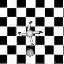
\includegraphics{images/ant_imgobs.png}
	\centering
	\caption{A sample image observation of the target environments}
\end{figure}\label{fig_ant_imgobs}

A basic task, namely "move0", is similar to the "Ant" environment in OpenAI Gym~\cite{openaigym} except an extra image observation as state. The agent is required to move toward a specific direction $g_0=(1,0)$, and the reward at each time-step is given by:
\begin{align}
r = v_g + 1-c_p-c_c
\end{align}
Where $v_g=v \cdot g_0$ is the "forward reward", which rewards the agent for moving toward the target direction. A sphere object presents in the environments at a constant distance from the robot agent to represent the target direction.  $c_p$ is the control cost, which is the power that the agent is consuming, and $c_c$ is the contact cost, which penalizes the agent for collisions. The episode terminates when the agent enters the unrecoverable state of being upside-down, or if the episode length reaches 1000 time-steps.

Apart from "move0", a set of similar tasks with different target directions are denoted as "move1", "move2", "move3", ..., "move7". This tasks are the same as "move0" except that the goal direction is different. The image observation is actually redundant for all these low-level tasks, because the agent only needs to move toward one specific direction in their corresponding environments.

Apart from these simple task, we also propose several tasks that has more complexity. We propose several multi-modality environments such as "moveg2", "moveg4", "moveg8", "movecont", "dynamicg8", "dynamiccont". These tasks requires the agent to learn not only from the state representation but also the image representation. We also propose sparse multi-modality environments, such as "reachcont". The agent receives sparse reward signals in these environments compared with the previous environments. The target direction or location is represented by a sphere object and can be seen in the image observation.
The set of all the proposed environments are described in details in table \ref{table_ant_envs}.


\begin{table}[!htbp]

\begin{center}
\begin{tabular}{|c|p{3cm}|p{4cm}|p{4cm}|}
\hline
Task name & Goal & Reward  &  Description \\
\hline\hline
move0 & velocity: $g_0=(1,0)$ &$ v_g+1-c_p-c_c$  & move toward a target direction \\
\hline
move1 & velocity: $g_1=(-1,0)$ &$ v_g+1-c_p-c_c$  & move toward a target direction\\
\hline
move2 & velocity: $g_2=(0,1)$ &$ v_g+1-c_p-c_c$  & move toward a target direction \\
\hline
move3 & velocity: $g_3=(0,-1)$ &$ v_g+1-c_p-c_c$  & move toward a target direction \\ 
\hline 
move4 & velocity: $g_4=(\sqrt{2}/2,\sqrt{2}/2)$ &$ v_g+1-c_p-c_c$  & move toward a target direction \\ 
\hline 
move5 & velocity: $g_5=(-\sqrt{2}/2,-\sqrt{2}/2)$ &$ v_g+1-c_p-c_c$  & move toward a target direction \\ 
\hline 
move6 & velocity: $g_6=(\sqrt{2}/2,-\sqrt{2}/2)$ &$ v_g+1-c_p-c_c$  & move toward a target direction \\ 
\hline 
move7 & velocity: $g_7=(-\sqrt{2}/2,\sqrt{2}/2)$ &$ v_g+1-c_p-c_c$  & move toward a target direction \\ 
\hline 
moveg2 & velocity samples from: $\{g_0,g_1\}$ &$ v_g+1-c_p-c_c$  & each episode has a random sampled target direction \\ \hline
moveg4 & velocity samples from: $\{g_0,g_1,g_2,g_3\}$ &$ v_g+1-c_p-c_c$  & each episode has a random sampled target direction \\ \hline
moveg8 & velocity samples from: $\{g_0,g_1, \dots,g_7\}$ &$ v_g+1-c_p-c_c$  & each episode has a random sampled target direction \\ \hline
movecont & velocity samples from a continuous range of all unit directions&$ v_g+1-c_p-c_c$  & each episode has a random sampled target direction \\ \hline
dynamicg8 &  velocity samples from: $\{g_0,g_1, \dots,g_7\}$ &$ v_g-c_p-c_c$  & the target direction is re-sampled with probability 0.005 at each time-step  \\ \hline
dynamiccont & velocity samples from a continuous range of all unit directions &$ v_g-c_p-c_c$  & the target direction is re-sampled with probability 0.005 at each time-step  \\ \hline
reachg4 & position samples from $\{g_0,g_1,g_2,g_3\}$ & $I(\lVert x-g\rVert_2^2<0.5) - 0.01$  & The agent is terminated when reaching a target position\\ \hline
reachcont & position samples from the unit circle & $I(\lVert x-g\rVert_2^2<0.5) - 0.01$  & The episode is terminated when reaching a target position\\ \hline
reachcontreg & position samples from the unit circle & $5I(\lVert x-g\rVert_2^2<0.5) - 0.01$  & A new target is sampled when the agent has reached the target position\\ \hline
\end{tabular}
\end{center}
 \caption{Summary of Ant-based environments}
\end{table}\label{table_ant_envs}
